\documentclass{beamer}

\usepackage{amssymb}

\title{FUN with Complexity: Walking through Doors is Hard, even without Staircases}
\author{Manuel Frohn}
\institute{RWTH Aachen}
\date{2024}

\begin{document}
\frame{\titlepage}
\begin{frame}
  \frametitle{Content}
  \tableofcontents
\end{frame}
%1
\section{Theory}
\subsection{PSPACE-Complexity}
\begin{frame}
  \frametitle{PSPACE-Complexity}
  A given problem requires a polynomial amount of memory in relation to the
  input, to be solved $\Leftrightarrow$ The problem is in PSPACE
  \\~\\
  \begin{minipage}[t]{0.48\textwidth}
    \textbf{SAT}
    \[ x_1 \land x_2 \lor \lnot x_3 \]
  \end{minipage}
  \begin{minipage}[t]{0.48\textwidth}
    \textbf{Quantified SAT}
    \[ \forall x_1 \exists x_2 : x_1 \land x_2 \lor \lnot x_3 \]
  \end{minipage}
\end{frame}
%2
\subsection{1-PlayerMotionPlaning}
\begin{frame}
  \frametitle{1-PlayerMotionPlaning}
  Given: Enviroment, Agent, Goal \\
  Question: Is the goal achivable
  \\~\\
  \centerline{
    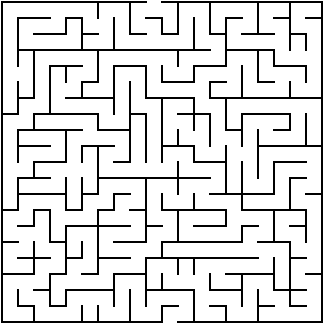
\includegraphics[width=0.40\textwidth]{res/Maze.png}
    \hspace{2.5cm}
    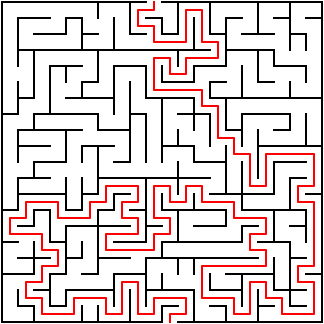
\includegraphics[width=0.40\textwidth]{res/MazeSolved.png}
  }
\end{frame}
%3
\subsection{Basic Door Device}
\begin{frame}
  \frametitle{Basic Door Device}
  \centerline{
    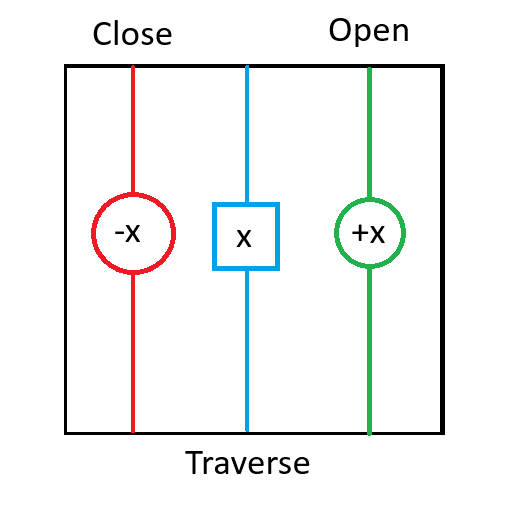
\includegraphics[width=0.40\textwidth]{res/Door.png}
    \hspace{2.5cm}
    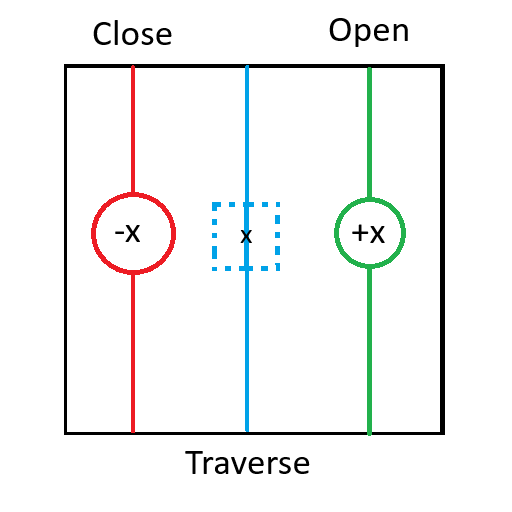
\includegraphics[width=0.40\textwidth]{res/DoorOpend.png}
  }
\end{frame}
%4
\subsection{PSPACE-hardness of doors}
\begin{frame}
  \frametitle{PSPACE-hardness of doors}
  \begin{theorem}
    If a game features \textbf{door devices} which each are controled by an
    \textcolor{green}{open} and a \textcolor{red}{close} \textbf{preasure plate}
    and the agent has to navigate from entrance to exit, then the game is
    \textbf{PSPACE-hard}
  \end{theorem}
\end{frame}
%5
\begin{frame}
  \frametitle{PSPACE-hardness of doors - Proof}
  \begin{minipage}[t]{0.48\textwidth}
    \textbf{True Quantified SAT}
    \[ \forall x \exists y \exists z :  (\overline{x} \lor y \lor z) \land \]
    \[ (\overline{x} \lor \overline{y} \lor z) \land (\lor x \lor y \lor \overline{z}) \]
  \end{minipage}
  \begin{minipage}[t]{0.48\textwidth}
    \textbf{1-Player Motion Planning}
    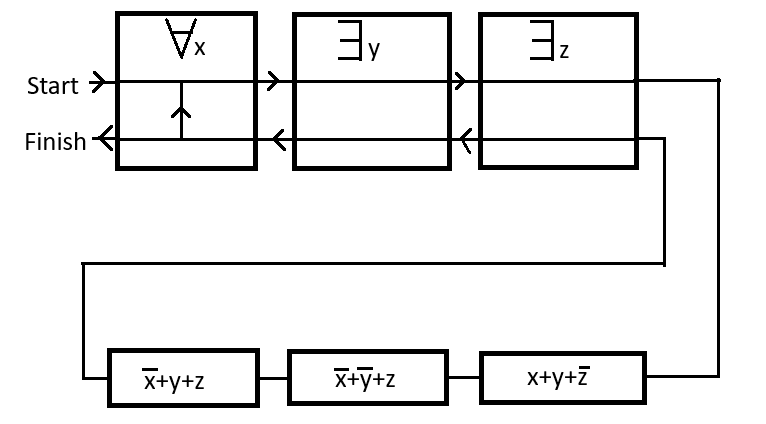
\includegraphics[width=1.20\textwidth]{res/Conversion.png}
  \end{minipage}
\end{frame}

%6
\begin{frame}
  \frametitle{PSPACE-hardness of doors - Proof}
  \begin{minipage}[t]{0.45\textwidth}
    \textbf{Clause}
    \[ (\overline{x} \lor y \lor z) \]
  \end{minipage}
  \begin{minipage}[t]{0.45\textwidth}
    \textbf{Gadget}
    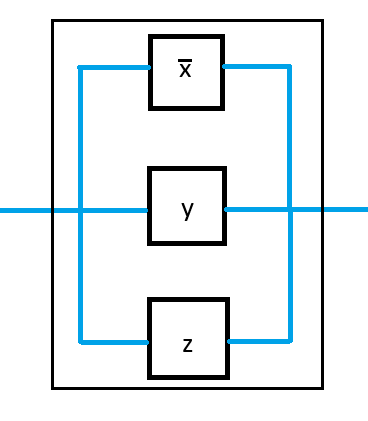
\includegraphics[width=0.9\textwidth]{res/ClauseGadget.png}
  \end{minipage}
\end{frame}

%7
\begin{frame}
  \frametitle{PSPACE-hardness of doors - Proof}
  \begin{minipage}[t]{0.45\textwidth}
    \textbf{Exists-Quantor}
    \[ \exists y \]
  \end{minipage}
  \begin{minipage}[t]{0.45\textwidth}
    \textbf{Gadget}
    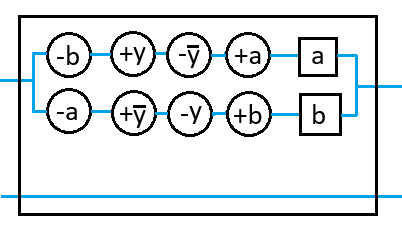
\includegraphics[width=1.3\textwidth]{res/ExsistsGadget.png}
  \end{minipage}
\end{frame}

%8
\begin{frame}
  \frametitle{PSPACE-hardness of doors - Proof}
  \begin{minipage}[t]{0.45\textwidth}
    \textbf{All-Quantor}
    \[ \forall x \]
  \end{minipage}
  \begin{minipage}[t]{0.45\textwidth}
    \textbf{Gadget}
    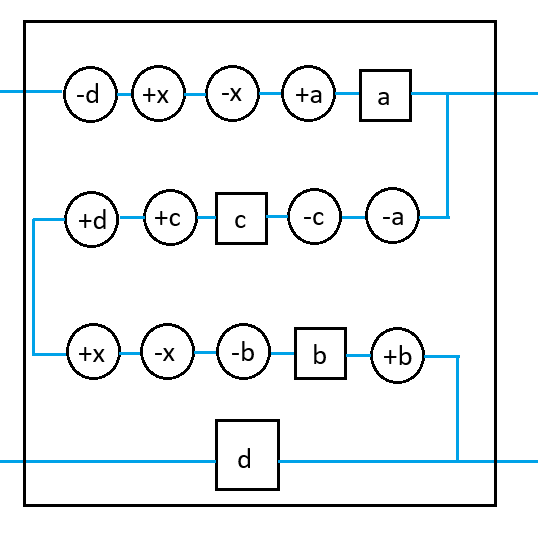
\includegraphics[width=1.3\textwidth]{res/AllGadget.png}
  \end{minipage}
\end{frame}

%9
\begin{frame}
  \frametitle{Door Device - Variants}
  \begin{minipage}[t]{0.32\textwidth}
    \textbf{Basic}
    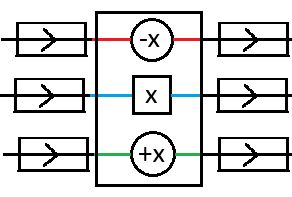
\includegraphics[width=1\textwidth]{res/DoorNormal.png}
  \end{minipage}
  \begin{minipage}[t]{0.32\textwidth}
    \textbf{Directed}
    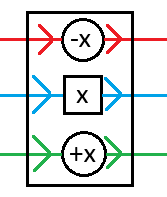
\includegraphics[width=1\textwidth]{res/DoorDirected.png}
  \end{minipage}
  \begin{minipage}[t]{0.32\textwidth}
    \textbf{Open-Optional}
    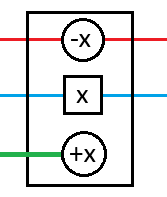
\includegraphics[width=1\textwidth]{res/DoorOpenOptional.png}
  \end{minipage}

\end{frame}

%10
\begin{frame}
  \frametitle{Self closing doors}
  \begin{minipage}[t]{0.49\textwidth}
    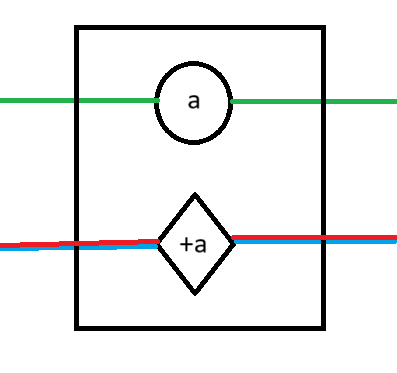
\includegraphics[width=1\textwidth]{res/SelfClosingDoor.png}
  \end{minipage}
  \begin{minipage}[t]{0.49\textwidth}
    \begin{itemize}
      \item Combines \textbf{close} and \textbf{traverse} tunnels into one
      \item Simpler
      \item More commen
    \end{itemize}
  \end{minipage}
\end{frame}

%11
\begin{frame}
  \frametitle{Self closing doors - Variants}

  \begin{minipage}[t]{0.32\textwidth}
    \textbf{Directed}
    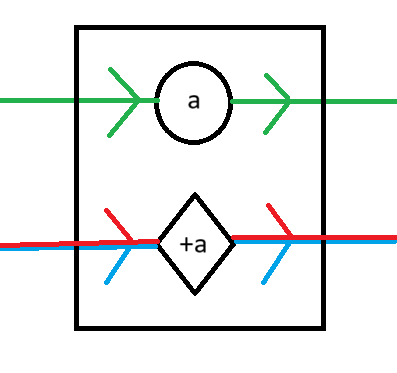
\includegraphics[width=1\textwidth]{res/SelfClosingDoorDirected.png}
  \end{minipage}
  \begin{minipage}[t]{0.32\textwidth}
    \textbf{Open-Optional}s 
    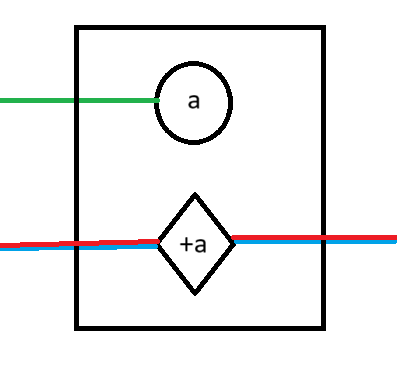
\includegraphics[width=1\textwidth]{res/SelfClosingDoorOpenOptional.png}
  \end{minipage}
  \begin{minipage}[t]{0.232\textwidth}
    \textbf{Symetric}
    % TODO one door should be always open
    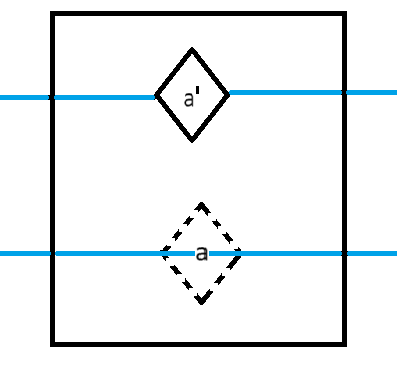
\includegraphics[width=1.3\textwidth]{res/SelfClosingSymetricDoor.png}
  \end{minipage}

\end{frame}
\end{document}